\section{Forward Time-Of-Flight (FTOF)}


\subsection{Geometry}

The FTOF geometry is implemented through the COATJAVA geometry service.
The service provides the geant4 definitions that are read by the GEMC perl api to build the geometry database.

All scintillators are geant4 volumes.
Each scintillator is a G4Box embedded in a G4Trapezoid mother volume made of air, see \F{ftofGeometry}.

\begin{figure}
	\centering
	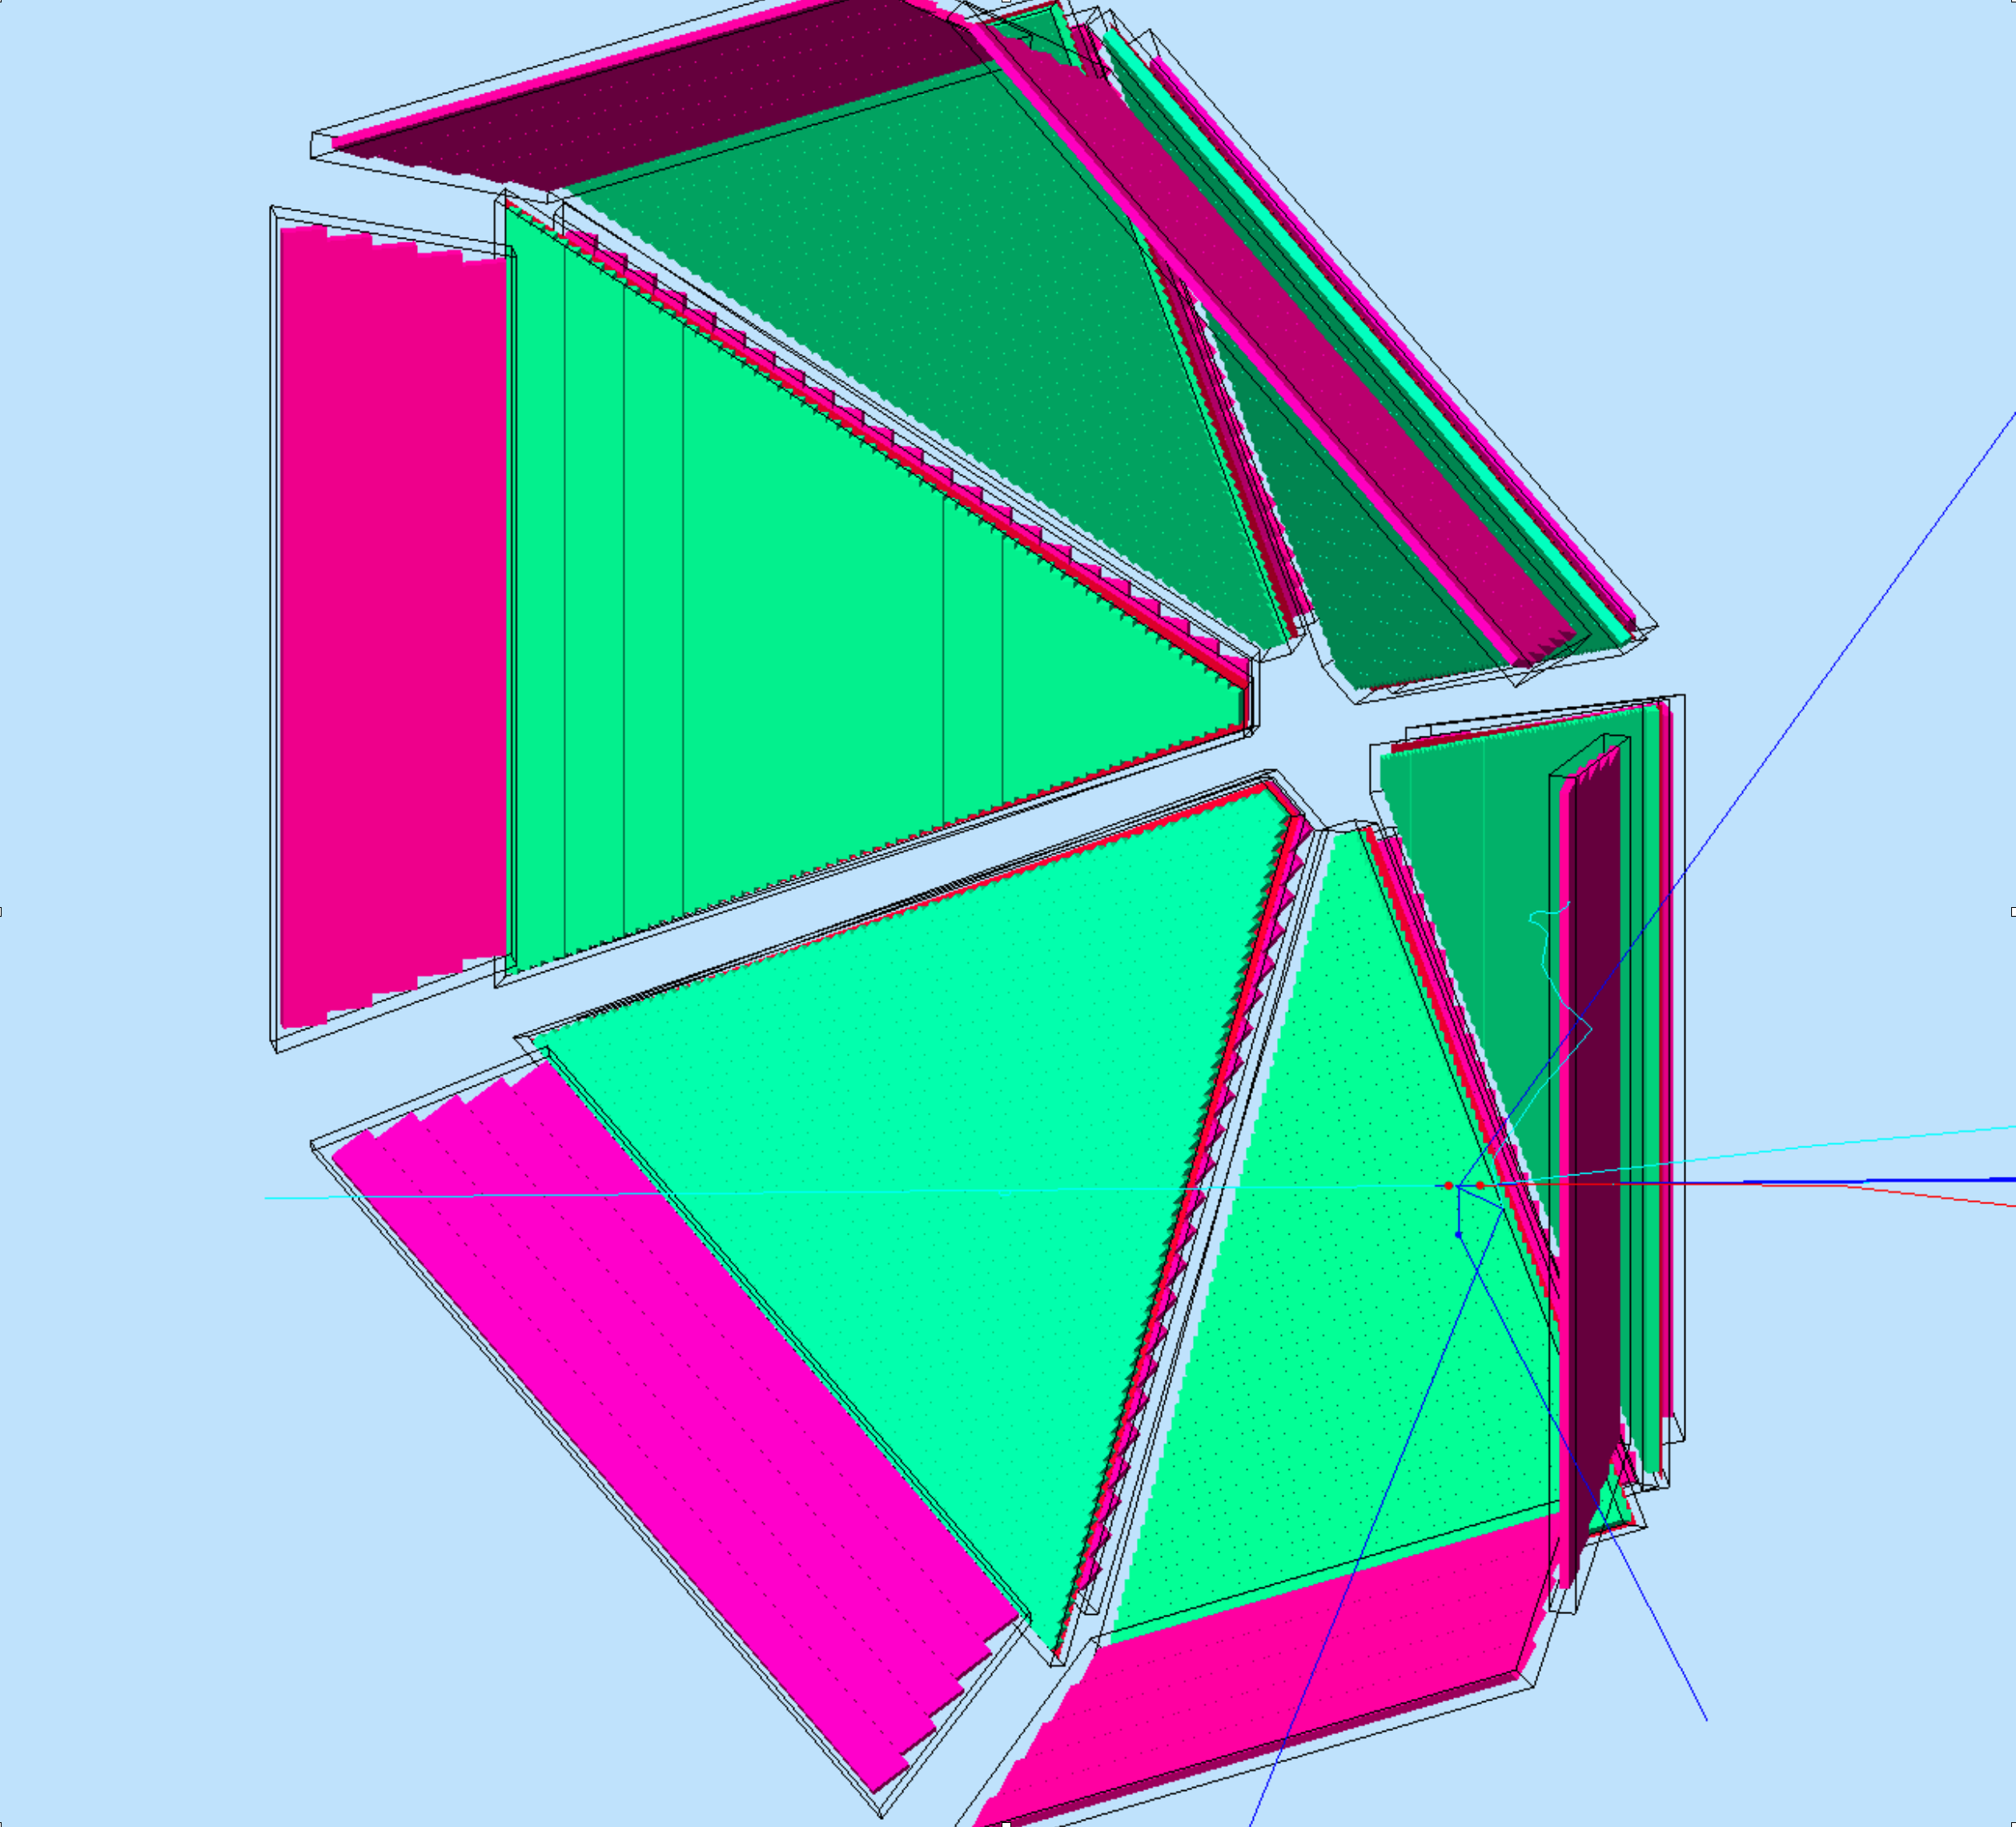
\includegraphics[width=0.95\columnwidth,keepaspectratio]{img/ftofGeometry.png}
	\caption{The GEMC implementation of the FTOF geomerty. The paddles are G4Boxes, embedded in trapezoid representing the mother volumes of each panel.}
	\label{fig:ftofGeometry}
\end{figure}


\subsubsection{Geometry Git Location}
The github location of the gemc perl api script is \url{https://github.com/gemc/detectors/tree/master/clas12/ftof}

\subsection{Process ID}
Each hit in the paddles is splitted in two identical hits with the identifier variable "side" sets to 0 (for the left side PMT) and 1 (for right side PMT).

\subsection{Digitization}

The energy deposited is reduced based on the position on the paddle using the calibration attenuation length. It is then

\subsubsection{Summary of CCDB Table used}
\begin{itemize}
	\item /calibration/ftof/attenuation
	\item /calibration/ftof/effective_velocity
	\item /calibration/ftof/effective_velocity
	\item /calibration/ftof/status
	\item /calibration/ftof/gain_balance
	\item /calibration/ftof/time_walk
	\item /calibration/ftof/time_offsets
	\item /calibration/ftof/tdc_conv
	\item /daq/tt/ftof
\end{itemize}

\subsection{Digitized Bank}
The output



\subsubsection{Time Window}

\subsubsection{Process Routine Git Repository Location}


